% ============================================================
% Lecture deck — Module 8 / Notebook 27
% LLM Fundamentals. HSBI house style. TikZ visuals.
% The notebook is the single source of truth.
% ============================================================
\documentclass[aspectratio=169,11pt]{beamer}

\usepackage[utf8]{inputenc}
\usepackage[T1]{fontenc}
\usepackage{lmodern}
\usepackage[english]{babel}
\usepackage{graphicx}
\usepackage{booktabs}
\usepackage{amsmath,amssymb}
\usepackage{xcolor}
\usepackage{tikz}
\usetikzlibrary{positioning,arrows.meta,shapes.geometric,calc,fit,backgrounds}

% Speaker notes. Default build = clean slides, unchanged. For presenter view
% (slide left, notes right) build with:
%   pdflatex "\def\notesmode{}% ============================================================
% Lecture deck — Module 8 / Notebook 27
% LLM Fundamentals. HSBI house style. TikZ visuals.
% The notebook is the single source of truth.
% ============================================================
\documentclass[aspectratio=169,11pt]{beamer}

\usepackage[utf8]{inputenc}
\usepackage[T1]{fontenc}
\usepackage{lmodern}
\usepackage[english]{babel}
\usepackage{graphicx}
\usepackage{booktabs}
\usepackage{amsmath,amssymb}
\usepackage{xcolor}
\usepackage{tikz}
\usetikzlibrary{positioning,arrows.meta,shapes.geometric,calc,fit,backgrounds}

% Speaker notes. Default build = clean slides, unchanged. For presenter view
% (slide left, notes right) build with:
%   pdflatex "\def\notesmode{}% ============================================================
% Lecture deck — Module 8 / Notebook 27
% LLM Fundamentals. HSBI house style. TikZ visuals.
% The notebook is the single source of truth.
% ============================================================
\documentclass[aspectratio=169,11pt]{beamer}

\usepackage[utf8]{inputenc}
\usepackage[T1]{fontenc}
\usepackage{lmodern}
\usepackage[english]{babel}
\usepackage{graphicx}
\usepackage{booktabs}
\usepackage{amsmath,amssymb}
\usepackage{xcolor}
\usepackage{tikz}
\usetikzlibrary{positioning,arrows.meta,shapes.geometric,calc,fit,backgrounds}

% Speaker notes. Default build = clean slides, unchanged. For presenter view
% (slide left, notes right) build with:
%   pdflatex "\def\notesmode{}% ============================================================
% Lecture deck — Module 8 / Notebook 27
% LLM Fundamentals. HSBI house style. TikZ visuals.
% The notebook is the single source of truth.
% ============================================================
\documentclass[aspectratio=169,11pt]{beamer}

\usepackage[utf8]{inputenc}
\usepackage[T1]{fontenc}
\usepackage{lmodern}
\usepackage[english]{babel}
\usepackage{graphicx}
\usepackage{booktabs}
\usepackage{amsmath,amssymb}
\usepackage{xcolor}
\usepackage{tikz}
\usetikzlibrary{positioning,arrows.meta,shapes.geometric,calc,fit,backgrounds}

% Speaker notes. Default build = clean slides, unchanged. For presenter view
% (slide left, notes right) build with:
%   pdflatex "\def\notesmode{}\input{27_llm_fundamentals.tex}"
\ifdefined\notesmode
  \usepackage{pgfpages}
  \setbeameroption{show notes on second screen=right}
\fi

\usetheme{Madrid}
\usecolortheme{default}
\setbeamertemplate{navigation symbols}{}
\setbeamertemplate{footline}[frame number]
\setbeamertemplate{blocks}[rounded][shadow=false]
\setbeamertemplate{headline}{%
  \leavevmode%
  \hbox{%
    \begin{beamercolorbox}[wd=\paperwidth,ht=2.5ex,dp=1.125ex]{section in head/foot}%
      \insertsectionnavigationhorizontal{\paperwidth}{}{\hskip0pt plus1filll}%
    \end{beamercolorbox}%
  }%
}
\AtBeginSection[]{%
  \begin{frame}{Outline}
    \tableofcontents[currentsection,sectionstyle=show/shaded,subsectionstyle=show/show/hide]
  \end{frame}
}

\definecolor{hsbiblue}{RGB}{45,57,120}
\definecolor{hsbimid}{RGB}{76,114,176}
\definecolor{hsbilight}{RGB}{225,231,247}
\definecolor{cgreen}{RGB}{85,164,103}
\definecolor{corange}{RGB}{221,132,82}
\definecolor{cred}{RGB}{196,78,82}
\definecolor{cpurple}{RGB}{129,114,178}
\tikzset{
  box/.style={rounded corners=3pt, draw=hsbiblue, line width=1pt, fill=hsbilight, align=center, inner sep=5pt, font=\footnotesize},
  tok/.style={rounded corners=2pt, draw=hsbiblue, line width=1pt, fill=hsbimid!22, align=center, minimum height=0.7cm, inner xsep=4pt, font=\footnotesize\ttfamily},
  arr/.style={-{Stealth[length=2.6mm]}, line width=1pt, draw=hsbiblue},
}

\title{LLM Fundamentals}
\subtitle{Module 8 --- AI Engineering $\cdot$ Notebook 27}
\author{Prof.\ Dr.\ Christoph Weisser}
\institute{HSBI}
\date{Summer Semester 2026}

\begin{document}

\begin{frame}\titlepage\end{frame}

\begin{frame}{Contents}
  \tableofcontents[hideallsubsections]
\end{frame}

% ============================================================
\section{Tokens}
% ============================================================
\begin{frame}{What is a Large Language Model?}
  \begin{block}{A next-token predictor}
    An LLM learns statistical relationships between words from massive corpora. Given some text, it computes the \emph{most probable continuation}, one token at a time.
  \end{block}
  \begin{exampleblock}{Analogy}
    Someone who has read every book ever written: they can continue any topic plausibly --- but have \emph{no built-in sense} of what is true, current, or private to your company.
  \end{exampleblock}
  \note{%
    \textbf{$\sim$6 min --- the framing for the whole lecture.}\\[2pt]
    Point: everything surprising about LLMs (hallucination, cutoff, prompt sensitivity) follows from \emph{one} fact --- it predicts the next token. Say that now; you will call back to it on every remaining slide.\\[2pt]
    \textbf{Ask the room:} ``If it only predicts likely text, why does it ever get facts right?'' Answer: true statements are common in the training data, so plausibility and truth correlate --- but only correlate. That gap is the entire second half of this lecture.\\[2pt]
    \textbf{Resist} defining tokens, attention or temperature here --- they each get their own slide.
  }
\end{frame}

\begin{frame}{How LLMs see text: tokens}
  \begin{center}
  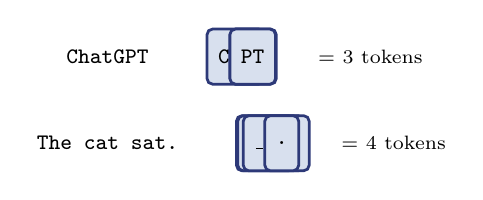
\begin{tikzpicture}[node distance=2pt]
    \node[font=\footnotesize] (l1) at (-3.0,0.55) {\texttt{ChatGPT}};
    \node[tok, right=0.6cm of l1] (t1) {Chat};
    \node[tok, right of=t1] (t2) {G};
    \node[tok, right of=t2] (t3) {PT};
    \node[font=\scriptsize, right=0.4cm of t3] {= 3 tokens};
    \node[font=\footnotesize] (l2) at (-3.0,-0.55) {\texttt{The cat sat.}};
    \node[tok, right=0.6cm of l2] (u1) {The};
    \node[tok, right of=u1] (u2) {\_cat};
    \node[tok, right of=u2] (u3) {\_sat};
    \node[tok, right of=u3] (u4) {.};
    \node[font=\scriptsize, right=0.4cm of u4] {= 4 tokens};
  \end{tikzpicture}
  \end{center}
  \begin{itemize}
    \item Cost and the \textbf{context window} are measured in tokens --- not characters, not words.
    \item Rule of thumb: 1 English token $\approx$ 4 characters $\approx$ 0.75 words ($1{,}000$ tokens $\approx$ 750 words).
    \item Code and non-English text tokenize \emph{less} efficiently; the model is blind to characters \emph{within} a token (``how many r's in strawberry?'').
  \end{itemize}
  \note{%
    \textbf{$\sim$10 min.} Point: tokens are the unit of \emph{cost}, \emph{context} and \emph{blindness}.\\[2pt]
    The strawberry example is the one they'll remember --- the model can't count letters it never sees separately. Ask it live if you have a provider configured; it fails convincingly.\\[2pt]
    \textbf{Ask the room:} ``Your prompt is 2{,}000 words. Roughly how many tokens, and does it fit?'' ($\approx$2{,}700 --- fits anywhere today.) The arithmetic matters because they'll be paying per token in Module 8.\\[2pt]
    \textbf{Non-English matters here:} German compounds tokenize badly, so the same text costs noticeably more than in English. Worth naming for a German-speaking cohort.
  }
\end{frame}

\begin{frame}{What are parameters? Why ``large''?}
  \small
  \begin{center}
  \begin{tabular}{llr}
    \toprule
    \textbf{Model} & \textbf{Parameters} & \textbf{Year} \\
    \midrule
    GPT-2                              & 1.5 billion                  & 2019 \\
    Llama-3 (open-weights)             & 8B / 70B / 405B              & 2024 \\
    Frontier (GPT-5.x, Claude, Gemini) & hundreds of billions (est.)  & 2023+ \\
    \bottomrule
  \end{tabular}
  \end{center}
  \begin{alertblock}{Key insight}
    There is \emph{no} manual list of facts inside the model. Knowledge is \emph{implicitly distributed} across all the weights --- which is exactly why it can be confidently wrong.
  \end{alertblock}
  \note{%
    \textbf{$\sim$7 min.} Point: parameters are learned weights, not stored facts. There is no row in a table saying ``Paris is the capital of France.''\\[2pt]
    That is \emph{why} you cannot patch a wrong fact by editing something, and why the fix is RAG (retrieval), not surgery on the model.\\[2pt]
    \textbf{Keep the numbers loose} --- frontier parameter counts are estimates and they date fast. The trend is the teaching point, not the figures.\\[2pt]
    \textbf{Ask the room:} ``Where inside the model is the fact stored?'' The honest answer --- smeared across billions of weights, nowhere in particular --- is genuinely unsettling and should be.
  }
\end{frame}

% ============================================================
\section{Training}
% ============================================================
\begin{frame}{The training objective: next-token prediction}
  \begin{block}{Hide $\to$ predict $\to$ measure $\to$ nudge, trillions of times}
    Hide the next token, ask the model to predict it, measure the error, nudge every parameter slightly toward a better prediction.
  \end{block}
  \[
    \mathcal{L} \;=\; -\sum_i y_i \log \hat{p}_i
  \]
  where $y_i = 1$ for the one true next token and $0$ otherwise (a \emph{one-hot} target), and $\hat{p}_i$ is the model's predicted probability for token $i$. Grammar, facts, and reasoning emerge as \emph{side-effects}.

  \vspace{2pt}
  {\footnotesize You write this exact loop --- loss $\to$ backward $\to$ step --- yourself in \textbf{Module 6 (PyTorch)}; an LLM trains with the same five moves, just with more parameters and more data.}
  \note{%
    \textbf{$\sim$10 min.} Point: the objective is embarrassingly simple, and everything impressive is a \emph{side-effect} of doing it at scale.\\[2pt]
    Don't derive the cross-entropy. Read it in words: ``the loss is small when the probability assigned to the token that actually came next is large.'' That sentence is the whole equation.\\[2pt]
    \textbf{The call-forward matters:} if your cohort is doing Module 6, promise them they will write this exact loop in PyTorch. It demystifies the whole thing --- same five moves, more data.\\[2pt]
    \textbf{Misconception to kill:} that the model was ``taught'' grammar or facts. Nobody labelled anything --- the text was its own label.
  }
\end{frame}

\begin{frame}{The output is a probability over \emph{every} token}
  \begin{center}
  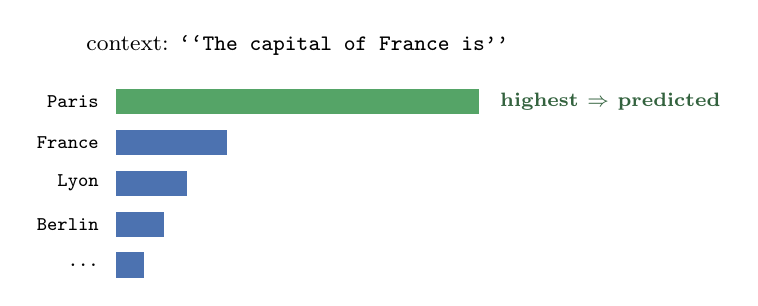
\begin{tikzpicture}
    \node[font=\footnotesize] at (2.4,0.7) {context: \texttt{``The capital of France is''}};
    \foreach \i/\tok/\p in {0/Paris/4.6, 1/France/1.4, 2/Lyon/0.9, 3/Berlin/0.6, 4/\ldots/0.35}{
      \node[left,font=\scriptsize\ttfamily] at (0,-\i*0.52) {\tok};
      \fill[hsbimid] (0.1,-\i*0.52-0.16) rectangle (0.1+\p,-\i*0.52+0.16);
    }
    \fill[cgreen] (0.1,0.16) rectangle (4.7,-0.16);  % highlight Paris (i=0)
    \node[right,font=\scriptsize\bfseries, cgreen!60!black] at (4.85,0) {highest $\Rightarrow$ predicted};
  \end{tikzpicture}
  \end{center}
  {\footnotesize The model never returns ``the answer'' --- it returns a \emph{distribution}. \texttt{temperature} controls how often it picks something other than the top token.}
  \note{%
    \textbf{$\sim$8 min.} Point: the output is a \emph{distribution}, not an answer. This is the slide that explains non-determinism.\\[2pt]
    \textbf{Ask the room:} ``You send the same prompt twice and get different answers. Bug or expected?'' Expected --- and controllable. temperature 0 takes the top token every time; higher temperature samples further down this bar chart.\\[2pt]
    Tie it to practice: \textbf{temperature 0 for extraction and classification} (you want the same answer twice), higher only when you want variety. They will set this parameter constantly from NB 28 onward.\\[2pt]
    Note that even at temperature 0 providers aren't perfectly reproducible --- batching and hardware introduce jitter. Mention only if asked; it's a rabbit hole.
  }
\end{frame}

% ============================================================
\section{Transformer}
% ============================================================
\begin{frame}{The architecture: the Transformer}
  \begin{block}{A stack of attention $+$ feed-forward layers}
    Each token becomes a vector; each layer lets tokens \emph{exchange information} (attention), then transforms each vector (feed-forward). Stack many layers $\to$ rich, context-aware representations.
  \end{block}
  \begin{itemize}
    \item All tokens are processed \emph{in parallel} during training --- a huge speed-up over older recurrent models.
    \item Depth (layers) $+$ width (vector size) $+$ data $=$ the ``large'' in LLM.
  \end{itemize}
  \note{%
    \textbf{$\sim$7 min.} Point: a stack of layers where tokens repeatedly \emph{look at each other} and then get transformed.\\[2pt]
    Pitch this at intuition level --- the next slide has the mechanics. The one structural fact worth stressing is \textbf{parallelism}: unlike the recurrent models it replaced, all tokens are processed at once, which is precisely what made training at this scale affordable.\\[2pt]
    \textbf{If the room is non-technical}, stop here and skip the Q/K/V slide entirely --- it is safely optional, and nothing later in the course depends on it.
  }
\end{frame}

\begin{frame}{The Attention mechanism (Q / K / V)}
  \small
  \begin{center}
  \begin{tabular}{ll}
    \toprule
    \textbf{Step} & \textbf{What happens} \\
    \midrule
    1. Project   & compute Query, Key, Value for every token via learned matrices \\
    2. Score     & $\mathrm{score}_{ij} = Q_i \cdot K_j / \sqrt{d_k}$ \\
    3. Normalise & softmax over $j$ $\to$ weights summing to 1 \\
    4. Mix       & new vector $= \sum_j \mathrm{weight}_{ij}\, V_j$ \\
    \bottomrule
  \end{tabular}
  \end{center}
  \vspace{2pt}
  {\footnotesize $d_k$ is the length of each Key/Query vector; dividing by $\sqrt{d_k}$ keeps scores from blowing up. \textbf{Intuition:} for each word, look at every other word and decide how much to listen to it.}
  \note{%
    \textbf{$\sim$12 min --- the most technical slide in the deck. Optional; cut it first if you are short on time.}\\[2pt]
    Lead with the intuition line at the bottom, \emph{then} the table --- not the other way round.\\[2pt]
    The analogy that works: Query = ``what am I looking for?'', Key = ``what do I offer?'', Value = ``what I actually contribute.'' Scoring Q against K is a relevance match; the softmax turns relevance into a weighting; the mix is a weighted average.\\[2pt]
    \textbf{Worked example on the board:} in ``The animal didn't cross the street because \emph{it} was too tired'', ask what ``it'' should attend to. Attention is what resolves that --- and the answer flips to ``street'' if you change ``tired'' to ``wide''.\\[2pt]
    Don't defend the $\sqrt{d_k}$; it's numerical hygiene, not insight.
  }
\end{frame}

% ============================================================
\section{Using LLMs}
% ============================================================
\begin{frame}{Three levels of using an LLM}
  \begin{center}
  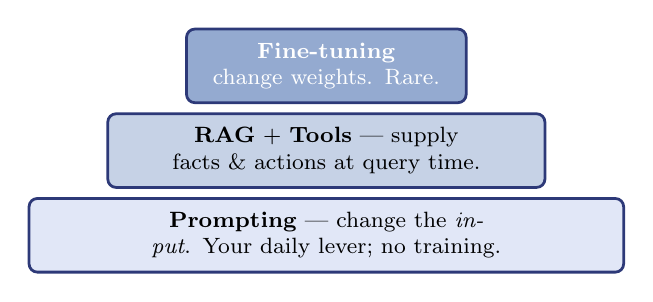
\begin{tikzpicture}
    \node[box, text width=7.2cm, fill=hsbilight]                         (b) {\textbf{Prompting} --- change the \emph{input}. Your daily lever; no training.};
    \node[box, text width=5.2cm, fill=hsbimid!32, above=3pt of b]        (m) {\textbf{RAG $+$ Tools} --- supply facts \& actions at query time.};
    \node[box, text width=3.2cm, fill=hsbimid!60, above=3pt of m, text=white] (t) {\textbf{Fine-tuning}\\ change weights. Rare.};
  \end{tikzpicture}
  \end{center}
  \begin{exampleblock}{Fine-tuning vs RAG}
    Fine-tuning changes \emph{behaviour / style}. \textbf{RAG} (NB 29) keeps the weights frozen and supplies \emph{fresh facts} --- don't fine-tune to add knowledge.
  \end{exampleblock}
  \note{%
    \textbf{$\sim$8 min.} Point: the pyramid is deliberately upside-down in effort --- the widest, cheapest lever (prompting) is the one you'll use 95\,\% of the time.\\[2pt]
    \textbf{The single most valuable correction in this lecture:} ``we'll fine-tune it on our documents'' is almost always wrong. Fine-tuning teaches \emph{behaviour and format}; it is a poor and expensive way to install \emph{facts}, which go stale the day after you train. Facts belong in retrieval.\\[2pt]
    \textbf{Ask the room:} ``You want the bot to answer from your 400-page handbook. Which level?'' RAG --- and if anyone says fine-tune, this is the moment to unpick it.\\[2pt]
    Forward-reference NB 29 (RAG) and NB 30 (tools) so it lands as a roadmap, not a taxonomy.
  }
\end{frame}

\begin{frame}{Five prompting techniques}
  \small
  \begin{center}
  \begin{tabular}{lp{7.0cm}}
    \toprule
    \textbf{Technique} & \textbf{When to reach for it} \\
    \midrule
    Zero-shot          & a general question; you trust the defaults \\
    Few-shot           & you want a \emph{consistent} format --- show 2--3 examples \\
    Chain-of-Thought   & multi-step reasoning --- ask it to work step by step \\
    Role assignment    & set tone / depth --- ``you are a senior analyst\ldots'' \\
    Format constraint  & machine-parseable output --- ``return JSON with keys\ldots'' \\
    \bottomrule
  \end{tabular}
  \end{center}
  {\footnotesize A production prompt stacks several: \emph{role} $+$ \emph{context} $+$ \emph{task} $+$ \emph{format} $+$ \emph{constraints}.}
  \note{%
    \textbf{$\sim$10 min --- make this the interactive one.}\\[2pt]
    Don't lecture the table. Take a deliberately bad prompt (``summarise this'') and improve it live with the room, adding one technique at a time until it's role $+$ context $+$ task $+$ format $+$ constraints. They should watch the output get sharper at each step.\\[2pt]
    \textbf{Format constraint is the one with engineering consequences:} ``return JSON with keys x, y'' is what makes an LLM callable as a \emph{function} rather than a chat toy --- that's the whole premise of NB 28.\\[2pt]
    Honest caveat on chain-of-thought: on newer reasoning models, explicitly asking for step-by-step adds less than it used to --- they already do it internally.
  }
\end{frame}

% ============================================================
\section{Limits}
% ============================================================
\begin{frame}{Two structural limitations}
  \begin{alertblock}{1. Hallucinations}
    The model predicts \emph{plausible} continuations, not \emph{true} ones --- so it can invent clauses, statistics, or APIs with full confidence.
  \end{alertblock}
  \begin{alertblock}{2. Knowledge cutoff}
    It knows nothing after its training date, and nothing about your \emph{private} data --- no current prices, no internal reports.
  \end{alertblock}
  \begin{exampleblock}{Mitigations (built later in the course)}
    \textbf{RAG} (NB 29) grounds answers in evidence $\cdot$ \textbf{Tools} (NB 30) let it look things up $\cdot$ \textbf{Evaluation} (NB 32) measures how often it's wrong.
  \end{exampleblock}
  \note{%
    \textbf{$\sim$10 min + close.} Point: both limitations are \emph{structural}, not bugs awaiting a patch --- they fall straight out of ``predicts plausible continuations.'' Close the loop with slide 1 explicitly.\\[2pt]
    Frame hallucination precisely: the model is not lying and does not know it is wrong. Nothing in the objective ever rewarded truth --- only plausibility.\\[2pt]
    \textbf{The professional habit to leave them with:} never ask ``is it accurate?'' --- ask ``\emph{how would I measure} how often it's wrong, and what happens when it is?'' That reframing is the bridge to NB 32 and to Module 18.\\[2pt]
    \textbf{Send them to Notebook 27} --- it runs entirely offline against the MockLLM, so nobody needs an API key to start.
  }
\end{frame}

\end{document}
"
\ifdefined\notesmode
  \usepackage{pgfpages}
  \setbeameroption{show notes on second screen=right}
\fi

\usetheme{Madrid}
\usecolortheme{default}
\setbeamertemplate{navigation symbols}{}
\setbeamertemplate{footline}[frame number]
\setbeamertemplate{blocks}[rounded][shadow=false]
\setbeamertemplate{headline}{%
  \leavevmode%
  \hbox{%
    \begin{beamercolorbox}[wd=\paperwidth,ht=2.5ex,dp=1.125ex]{section in head/foot}%
      \insertsectionnavigationhorizontal{\paperwidth}{}{\hskip0pt plus1filll}%
    \end{beamercolorbox}%
  }%
}
\AtBeginSection[]{%
  \begin{frame}{Outline}
    \tableofcontents[currentsection,sectionstyle=show/shaded,subsectionstyle=show/show/hide]
  \end{frame}
}

\definecolor{hsbiblue}{RGB}{45,57,120}
\definecolor{hsbimid}{RGB}{76,114,176}
\definecolor{hsbilight}{RGB}{225,231,247}
\definecolor{cgreen}{RGB}{85,164,103}
\definecolor{corange}{RGB}{221,132,82}
\definecolor{cred}{RGB}{196,78,82}
\definecolor{cpurple}{RGB}{129,114,178}
\tikzset{
  box/.style={rounded corners=3pt, draw=hsbiblue, line width=1pt, fill=hsbilight, align=center, inner sep=5pt, font=\footnotesize},
  tok/.style={rounded corners=2pt, draw=hsbiblue, line width=1pt, fill=hsbimid!22, align=center, minimum height=0.7cm, inner xsep=4pt, font=\footnotesize\ttfamily},
  arr/.style={-{Stealth[length=2.6mm]}, line width=1pt, draw=hsbiblue},
}

\title{LLM Fundamentals}
\subtitle{Module 8 --- AI Engineering $\cdot$ Notebook 27}
\author{Prof.\ Dr.\ Christoph Weisser}
\institute{HSBI}
\date{Summer Semester 2026}

\begin{document}

\begin{frame}\titlepage\end{frame}

\begin{frame}{Contents}
  \tableofcontents[hideallsubsections]
\end{frame}

% ============================================================
\section{Tokens}
% ============================================================
\begin{frame}{What is a Large Language Model?}
  \begin{block}{A next-token predictor}
    An LLM learns statistical relationships between words from massive corpora. Given some text, it computes the \emph{most probable continuation}, one token at a time.
  \end{block}
  \begin{exampleblock}{Analogy}
    Someone who has read every book ever written: they can continue any topic plausibly --- but have \emph{no built-in sense} of what is true, current, or private to your company.
  \end{exampleblock}
  \note{%
    \textbf{$\sim$6 min --- the framing for the whole lecture.}\\[2pt]
    Point: everything surprising about LLMs (hallucination, cutoff, prompt sensitivity) follows from \emph{one} fact --- it predicts the next token. Say that now; you will call back to it on every remaining slide.\\[2pt]
    \textbf{Ask the room:} ``If it only predicts likely text, why does it ever get facts right?'' Answer: true statements are common in the training data, so plausibility and truth correlate --- but only correlate. That gap is the entire second half of this lecture.\\[2pt]
    \textbf{Resist} defining tokens, attention or temperature here --- they each get their own slide.
  }
\end{frame}

\begin{frame}{How LLMs see text: tokens}
  \begin{center}
  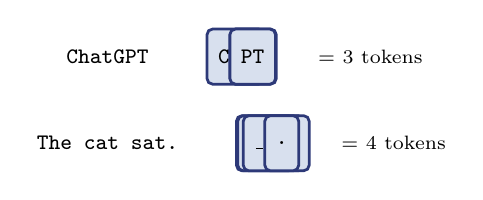
\begin{tikzpicture}[node distance=2pt]
    \node[font=\footnotesize] (l1) at (-3.0,0.55) {\texttt{ChatGPT}};
    \node[tok, right=0.6cm of l1] (t1) {Chat};
    \node[tok, right of=t1] (t2) {G};
    \node[tok, right of=t2] (t3) {PT};
    \node[font=\scriptsize, right=0.4cm of t3] {= 3 tokens};
    \node[font=\footnotesize] (l2) at (-3.0,-0.55) {\texttt{The cat sat.}};
    \node[tok, right=0.6cm of l2] (u1) {The};
    \node[tok, right of=u1] (u2) {\_cat};
    \node[tok, right of=u2] (u3) {\_sat};
    \node[tok, right of=u3] (u4) {.};
    \node[font=\scriptsize, right=0.4cm of u4] {= 4 tokens};
  \end{tikzpicture}
  \end{center}
  \begin{itemize}
    \item Cost and the \textbf{context window} are measured in tokens --- not characters, not words.
    \item Rule of thumb: 1 English token $\approx$ 4 characters $\approx$ 0.75 words ($1{,}000$ tokens $\approx$ 750 words).
    \item Code and non-English text tokenize \emph{less} efficiently; the model is blind to characters \emph{within} a token (``how many r's in strawberry?'').
  \end{itemize}
  \note{%
    \textbf{$\sim$10 min.} Point: tokens are the unit of \emph{cost}, \emph{context} and \emph{blindness}.\\[2pt]
    The strawberry example is the one they'll remember --- the model can't count letters it never sees separately. Ask it live if you have a provider configured; it fails convincingly.\\[2pt]
    \textbf{Ask the room:} ``Your prompt is 2{,}000 words. Roughly how many tokens, and does it fit?'' ($\approx$2{,}700 --- fits anywhere today.) The arithmetic matters because they'll be paying per token in Module 8.\\[2pt]
    \textbf{Non-English matters here:} German compounds tokenize badly, so the same text costs noticeably more than in English. Worth naming for a German-speaking cohort.
  }
\end{frame}

\begin{frame}{What are parameters? Why ``large''?}
  \small
  \begin{center}
  \begin{tabular}{llr}
    \toprule
    \textbf{Model} & \textbf{Parameters} & \textbf{Year} \\
    \midrule
    GPT-2                              & 1.5 billion                  & 2019 \\
    Llama-3 (open-weights)             & 8B / 70B / 405B              & 2024 \\
    Frontier (GPT-5.x, Claude, Gemini) & hundreds of billions (est.)  & 2023+ \\
    \bottomrule
  \end{tabular}
  \end{center}
  \begin{alertblock}{Key insight}
    There is \emph{no} manual list of facts inside the model. Knowledge is \emph{implicitly distributed} across all the weights --- which is exactly why it can be confidently wrong.
  \end{alertblock}
  \note{%
    \textbf{$\sim$7 min.} Point: parameters are learned weights, not stored facts. There is no row in a table saying ``Paris is the capital of France.''\\[2pt]
    That is \emph{why} you cannot patch a wrong fact by editing something, and why the fix is RAG (retrieval), not surgery on the model.\\[2pt]
    \textbf{Keep the numbers loose} --- frontier parameter counts are estimates and they date fast. The trend is the teaching point, not the figures.\\[2pt]
    \textbf{Ask the room:} ``Where inside the model is the fact stored?'' The honest answer --- smeared across billions of weights, nowhere in particular --- is genuinely unsettling and should be.
  }
\end{frame}

% ============================================================
\section{Training}
% ============================================================
\begin{frame}{The training objective: next-token prediction}
  \begin{block}{Hide $\to$ predict $\to$ measure $\to$ nudge, trillions of times}
    Hide the next token, ask the model to predict it, measure the error, nudge every parameter slightly toward a better prediction.
  \end{block}
  \[
    \mathcal{L} \;=\; -\sum_i y_i \log \hat{p}_i
  \]
  where $y_i = 1$ for the one true next token and $0$ otherwise (a \emph{one-hot} target), and $\hat{p}_i$ is the model's predicted probability for token $i$. Grammar, facts, and reasoning emerge as \emph{side-effects}.

  \vspace{2pt}
  {\footnotesize You write this exact loop --- loss $\to$ backward $\to$ step --- yourself in \textbf{Module 6 (PyTorch)}; an LLM trains with the same five moves, just with more parameters and more data.}
  \note{%
    \textbf{$\sim$10 min.} Point: the objective is embarrassingly simple, and everything impressive is a \emph{side-effect} of doing it at scale.\\[2pt]
    Don't derive the cross-entropy. Read it in words: ``the loss is small when the probability assigned to the token that actually came next is large.'' That sentence is the whole equation.\\[2pt]
    \textbf{The call-forward matters:} if your cohort is doing Module 6, promise them they will write this exact loop in PyTorch. It demystifies the whole thing --- same five moves, more data.\\[2pt]
    \textbf{Misconception to kill:} that the model was ``taught'' grammar or facts. Nobody labelled anything --- the text was its own label.
  }
\end{frame}

\begin{frame}{The output is a probability over \emph{every} token}
  \begin{center}
  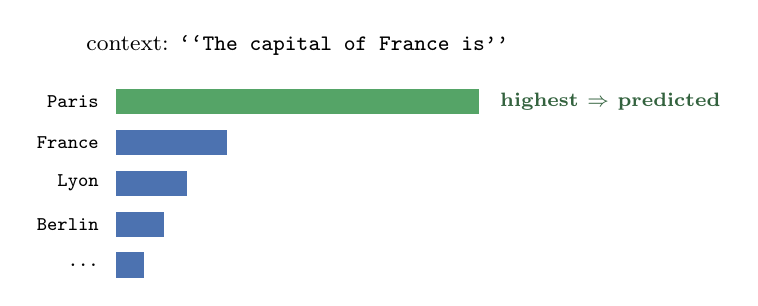
\begin{tikzpicture}
    \node[font=\footnotesize] at (2.4,0.7) {context: \texttt{``The capital of France is''}};
    \foreach \i/\tok/\p in {0/Paris/4.6, 1/France/1.4, 2/Lyon/0.9, 3/Berlin/0.6, 4/\ldots/0.35}{
      \node[left,font=\scriptsize\ttfamily] at (0,-\i*0.52) {\tok};
      \fill[hsbimid] (0.1,-\i*0.52-0.16) rectangle (0.1+\p,-\i*0.52+0.16);
    }
    \fill[cgreen] (0.1,0.16) rectangle (4.7,-0.16);  % highlight Paris (i=0)
    \node[right,font=\scriptsize\bfseries, cgreen!60!black] at (4.85,0) {highest $\Rightarrow$ predicted};
  \end{tikzpicture}
  \end{center}
  {\footnotesize The model never returns ``the answer'' --- it returns a \emph{distribution}. \texttt{temperature} controls how often it picks something other than the top token.}
  \note{%
    \textbf{$\sim$8 min.} Point: the output is a \emph{distribution}, not an answer. This is the slide that explains non-determinism.\\[2pt]
    \textbf{Ask the room:} ``You send the same prompt twice and get different answers. Bug or expected?'' Expected --- and controllable. temperature 0 takes the top token every time; higher temperature samples further down this bar chart.\\[2pt]
    Tie it to practice: \textbf{temperature 0 for extraction and classification} (you want the same answer twice), higher only when you want variety. They will set this parameter constantly from NB 28 onward.\\[2pt]
    Note that even at temperature 0 providers aren't perfectly reproducible --- batching and hardware introduce jitter. Mention only if asked; it's a rabbit hole.
  }
\end{frame}

% ============================================================
\section{Transformer}
% ============================================================
\begin{frame}{The architecture: the Transformer}
  \begin{block}{A stack of attention $+$ feed-forward layers}
    Each token becomes a vector; each layer lets tokens \emph{exchange information} (attention), then transforms each vector (feed-forward). Stack many layers $\to$ rich, context-aware representations.
  \end{block}
  \begin{itemize}
    \item All tokens are processed \emph{in parallel} during training --- a huge speed-up over older recurrent models.
    \item Depth (layers) $+$ width (vector size) $+$ data $=$ the ``large'' in LLM.
  \end{itemize}
  \note{%
    \textbf{$\sim$7 min.} Point: a stack of layers where tokens repeatedly \emph{look at each other} and then get transformed.\\[2pt]
    Pitch this at intuition level --- the next slide has the mechanics. The one structural fact worth stressing is \textbf{parallelism}: unlike the recurrent models it replaced, all tokens are processed at once, which is precisely what made training at this scale affordable.\\[2pt]
    \textbf{If the room is non-technical}, stop here and skip the Q/K/V slide entirely --- it is safely optional, and nothing later in the course depends on it.
  }
\end{frame}

\begin{frame}{The Attention mechanism (Q / K / V)}
  \small
  \begin{center}
  \begin{tabular}{ll}
    \toprule
    \textbf{Step} & \textbf{What happens} \\
    \midrule
    1. Project   & compute Query, Key, Value for every token via learned matrices \\
    2. Score     & $\mathrm{score}_{ij} = Q_i \cdot K_j / \sqrt{d_k}$ \\
    3. Normalise & softmax over $j$ $\to$ weights summing to 1 \\
    4. Mix       & new vector $= \sum_j \mathrm{weight}_{ij}\, V_j$ \\
    \bottomrule
  \end{tabular}
  \end{center}
  \vspace{2pt}
  {\footnotesize $d_k$ is the length of each Key/Query vector; dividing by $\sqrt{d_k}$ keeps scores from blowing up. \textbf{Intuition:} for each word, look at every other word and decide how much to listen to it.}
  \note{%
    \textbf{$\sim$12 min --- the most technical slide in the deck. Optional; cut it first if you are short on time.}\\[2pt]
    Lead with the intuition line at the bottom, \emph{then} the table --- not the other way round.\\[2pt]
    The analogy that works: Query = ``what am I looking for?'', Key = ``what do I offer?'', Value = ``what I actually contribute.'' Scoring Q against K is a relevance match; the softmax turns relevance into a weighting; the mix is a weighted average.\\[2pt]
    \textbf{Worked example on the board:} in ``The animal didn't cross the street because \emph{it} was too tired'', ask what ``it'' should attend to. Attention is what resolves that --- and the answer flips to ``street'' if you change ``tired'' to ``wide''.\\[2pt]
    Don't defend the $\sqrt{d_k}$; it's numerical hygiene, not insight.
  }
\end{frame}

% ============================================================
\section{Using LLMs}
% ============================================================
\begin{frame}{Three levels of using an LLM}
  \begin{center}
  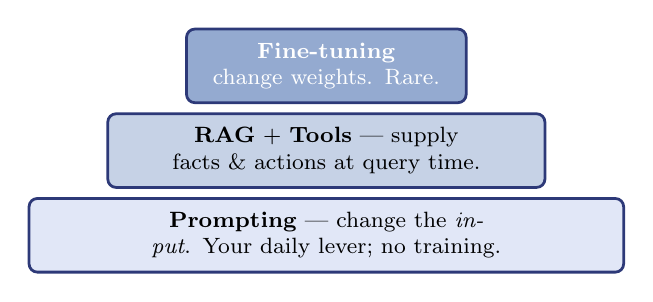
\begin{tikzpicture}
    \node[box, text width=7.2cm, fill=hsbilight]                         (b) {\textbf{Prompting} --- change the \emph{input}. Your daily lever; no training.};
    \node[box, text width=5.2cm, fill=hsbimid!32, above=3pt of b]        (m) {\textbf{RAG $+$ Tools} --- supply facts \& actions at query time.};
    \node[box, text width=3.2cm, fill=hsbimid!60, above=3pt of m, text=white] (t) {\textbf{Fine-tuning}\\ change weights. Rare.};
  \end{tikzpicture}
  \end{center}
  \begin{exampleblock}{Fine-tuning vs RAG}
    Fine-tuning changes \emph{behaviour / style}. \textbf{RAG} (NB 29) keeps the weights frozen and supplies \emph{fresh facts} --- don't fine-tune to add knowledge.
  \end{exampleblock}
  \note{%
    \textbf{$\sim$8 min.} Point: the pyramid is deliberately upside-down in effort --- the widest, cheapest lever (prompting) is the one you'll use 95\,\% of the time.\\[2pt]
    \textbf{The single most valuable correction in this lecture:} ``we'll fine-tune it on our documents'' is almost always wrong. Fine-tuning teaches \emph{behaviour and format}; it is a poor and expensive way to install \emph{facts}, which go stale the day after you train. Facts belong in retrieval.\\[2pt]
    \textbf{Ask the room:} ``You want the bot to answer from your 400-page handbook. Which level?'' RAG --- and if anyone says fine-tune, this is the moment to unpick it.\\[2pt]
    Forward-reference NB 29 (RAG) and NB 30 (tools) so it lands as a roadmap, not a taxonomy.
  }
\end{frame}

\begin{frame}{Five prompting techniques}
  \small
  \begin{center}
  \begin{tabular}{lp{7.0cm}}
    \toprule
    \textbf{Technique} & \textbf{When to reach for it} \\
    \midrule
    Zero-shot          & a general question; you trust the defaults \\
    Few-shot           & you want a \emph{consistent} format --- show 2--3 examples \\
    Chain-of-Thought   & multi-step reasoning --- ask it to work step by step \\
    Role assignment    & set tone / depth --- ``you are a senior analyst\ldots'' \\
    Format constraint  & machine-parseable output --- ``return JSON with keys\ldots'' \\
    \bottomrule
  \end{tabular}
  \end{center}
  {\footnotesize A production prompt stacks several: \emph{role} $+$ \emph{context} $+$ \emph{task} $+$ \emph{format} $+$ \emph{constraints}.}
  \note{%
    \textbf{$\sim$10 min --- make this the interactive one.}\\[2pt]
    Don't lecture the table. Take a deliberately bad prompt (``summarise this'') and improve it live with the room, adding one technique at a time until it's role $+$ context $+$ task $+$ format $+$ constraints. They should watch the output get sharper at each step.\\[2pt]
    \textbf{Format constraint is the one with engineering consequences:} ``return JSON with keys x, y'' is what makes an LLM callable as a \emph{function} rather than a chat toy --- that's the whole premise of NB 28.\\[2pt]
    Honest caveat on chain-of-thought: on newer reasoning models, explicitly asking for step-by-step adds less than it used to --- they already do it internally.
  }
\end{frame}

% ============================================================
\section{Limits}
% ============================================================
\begin{frame}{Two structural limitations}
  \begin{alertblock}{1. Hallucinations}
    The model predicts \emph{plausible} continuations, not \emph{true} ones --- so it can invent clauses, statistics, or APIs with full confidence.
  \end{alertblock}
  \begin{alertblock}{2. Knowledge cutoff}
    It knows nothing after its training date, and nothing about your \emph{private} data --- no current prices, no internal reports.
  \end{alertblock}
  \begin{exampleblock}{Mitigations (built later in the course)}
    \textbf{RAG} (NB 29) grounds answers in evidence $\cdot$ \textbf{Tools} (NB 30) let it look things up $\cdot$ \textbf{Evaluation} (NB 32) measures how often it's wrong.
  \end{exampleblock}
  \note{%
    \textbf{$\sim$10 min + close.} Point: both limitations are \emph{structural}, not bugs awaiting a patch --- they fall straight out of ``predicts plausible continuations.'' Close the loop with slide 1 explicitly.\\[2pt]
    Frame hallucination precisely: the model is not lying and does not know it is wrong. Nothing in the objective ever rewarded truth --- only plausibility.\\[2pt]
    \textbf{The professional habit to leave them with:} never ask ``is it accurate?'' --- ask ``\emph{how would I measure} how often it's wrong, and what happens when it is?'' That reframing is the bridge to NB 32 and to Module 18.\\[2pt]
    \textbf{Send them to Notebook 27} --- it runs entirely offline against the MockLLM, so nobody needs an API key to start.
  }
\end{frame}

\end{document}
"
\ifdefined\notesmode
  \usepackage{pgfpages}
  \setbeameroption{show notes on second screen=right}
\fi

\usetheme{Madrid}
\usecolortheme{default}
\setbeamertemplate{navigation symbols}{}
\setbeamertemplate{footline}[frame number]
\setbeamertemplate{blocks}[rounded][shadow=false]
\setbeamertemplate{headline}{%
  \leavevmode%
  \hbox{%
    \begin{beamercolorbox}[wd=\paperwidth,ht=2.5ex,dp=1.125ex]{section in head/foot}%
      \insertsectionnavigationhorizontal{\paperwidth}{}{\hskip0pt plus1filll}%
    \end{beamercolorbox}%
  }%
}
\AtBeginSection[]{%
  \begin{frame}{Outline}
    \tableofcontents[currentsection,sectionstyle=show/shaded,subsectionstyle=show/show/hide]
  \end{frame}
}

\definecolor{hsbiblue}{RGB}{45,57,120}
\definecolor{hsbimid}{RGB}{76,114,176}
\definecolor{hsbilight}{RGB}{225,231,247}
\definecolor{cgreen}{RGB}{85,164,103}
\definecolor{corange}{RGB}{221,132,82}
\definecolor{cred}{RGB}{196,78,82}
\definecolor{cpurple}{RGB}{129,114,178}
\tikzset{
  box/.style={rounded corners=3pt, draw=hsbiblue, line width=1pt, fill=hsbilight, align=center, inner sep=5pt, font=\footnotesize},
  tok/.style={rounded corners=2pt, draw=hsbiblue, line width=1pt, fill=hsbimid!22, align=center, minimum height=0.7cm, inner xsep=4pt, font=\footnotesize\ttfamily},
  arr/.style={-{Stealth[length=2.6mm]}, line width=1pt, draw=hsbiblue},
}

\title{LLM Fundamentals}
\subtitle{Module 8 --- AI Engineering $\cdot$ Notebook 27}
\author{Prof.\ Dr.\ Christoph Weisser}
\institute{HSBI}
\date{Summer Semester 2026}

\begin{document}

\begin{frame}\titlepage\end{frame}

\begin{frame}{Contents}
  \tableofcontents[hideallsubsections]
\end{frame}

% ============================================================
\section{Tokens}
% ============================================================
\begin{frame}{What is a Large Language Model?}
  \begin{block}{A next-token predictor}
    An LLM learns statistical relationships between words from massive corpora. Given some text, it computes the \emph{most probable continuation}, one token at a time.
  \end{block}
  \begin{exampleblock}{Analogy}
    Someone who has read every book ever written: they can continue any topic plausibly --- but have \emph{no built-in sense} of what is true, current, or private to your company.
  \end{exampleblock}
  \note{%
    \textbf{$\sim$6 min --- the framing for the whole lecture.}\\[2pt]
    Point: everything surprising about LLMs (hallucination, cutoff, prompt sensitivity) follows from \emph{one} fact --- it predicts the next token. Say that now; you will call back to it on every remaining slide.\\[2pt]
    \textbf{Ask the room:} ``If it only predicts likely text, why does it ever get facts right?'' Answer: true statements are common in the training data, so plausibility and truth correlate --- but only correlate. That gap is the entire second half of this lecture.\\[2pt]
    \textbf{Resist} defining tokens, attention or temperature here --- they each get their own slide.
  }
\end{frame}

\begin{frame}{How LLMs see text: tokens}
  \begin{center}
  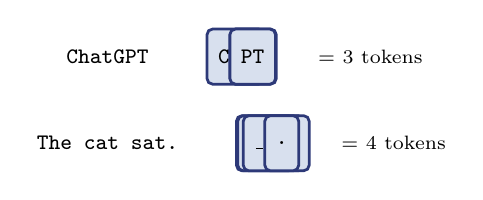
\begin{tikzpicture}[node distance=2pt]
    \node[font=\footnotesize] (l1) at (-3.0,0.55) {\texttt{ChatGPT}};
    \node[tok, right=0.6cm of l1] (t1) {Chat};
    \node[tok, right of=t1] (t2) {G};
    \node[tok, right of=t2] (t3) {PT};
    \node[font=\scriptsize, right=0.4cm of t3] {= 3 tokens};
    \node[font=\footnotesize] (l2) at (-3.0,-0.55) {\texttt{The cat sat.}};
    \node[tok, right=0.6cm of l2] (u1) {The};
    \node[tok, right of=u1] (u2) {\_cat};
    \node[tok, right of=u2] (u3) {\_sat};
    \node[tok, right of=u3] (u4) {.};
    \node[font=\scriptsize, right=0.4cm of u4] {= 4 tokens};
  \end{tikzpicture}
  \end{center}
  \begin{itemize}
    \item Cost and the \textbf{context window} are measured in tokens --- not characters, not words.
    \item Rule of thumb: 1 English token $\approx$ 4 characters $\approx$ 0.75 words ($1{,}000$ tokens $\approx$ 750 words).
    \item Code and non-English text tokenize \emph{less} efficiently; the model is blind to characters \emph{within} a token (``how many r's in strawberry?'').
  \end{itemize}
  \note{%
    \textbf{$\sim$10 min.} Point: tokens are the unit of \emph{cost}, \emph{context} and \emph{blindness}.\\[2pt]
    The strawberry example is the one they'll remember --- the model can't count letters it never sees separately. Ask it live if you have a provider configured; it fails convincingly.\\[2pt]
    \textbf{Ask the room:} ``Your prompt is 2{,}000 words. Roughly how many tokens, and does it fit?'' ($\approx$2{,}700 --- fits anywhere today.) The arithmetic matters because they'll be paying per token in Module 8.\\[2pt]
    \textbf{Non-English matters here:} German compounds tokenize badly, so the same text costs noticeably more than in English. Worth naming for a German-speaking cohort.
  }
\end{frame}

\begin{frame}{What are parameters? Why ``large''?}
  \small
  \begin{center}
  \begin{tabular}{llr}
    \toprule
    \textbf{Model} & \textbf{Parameters} & \textbf{Year} \\
    \midrule
    GPT-2                              & 1.5 billion                  & 2019 \\
    Llama-3 (open-weights)             & 8B / 70B / 405B              & 2024 \\
    Frontier (GPT-5.x, Claude, Gemini) & hundreds of billions (est.)  & 2023+ \\
    \bottomrule
  \end{tabular}
  \end{center}
  \begin{alertblock}{Key insight}
    There is \emph{no} manual list of facts inside the model. Knowledge is \emph{implicitly distributed} across all the weights --- which is exactly why it can be confidently wrong.
  \end{alertblock}
  \note{%
    \textbf{$\sim$7 min.} Point: parameters are learned weights, not stored facts. There is no row in a table saying ``Paris is the capital of France.''\\[2pt]
    That is \emph{why} you cannot patch a wrong fact by editing something, and why the fix is RAG (retrieval), not surgery on the model.\\[2pt]
    \textbf{Keep the numbers loose} --- frontier parameter counts are estimates and they date fast. The trend is the teaching point, not the figures.\\[2pt]
    \textbf{Ask the room:} ``Where inside the model is the fact stored?'' The honest answer --- smeared across billions of weights, nowhere in particular --- is genuinely unsettling and should be.
  }
\end{frame}

% ============================================================
\section{Training}
% ============================================================
\begin{frame}{The training objective: next-token prediction}
  \begin{block}{Hide $\to$ predict $\to$ measure $\to$ nudge, trillions of times}
    Hide the next token, ask the model to predict it, measure the error, nudge every parameter slightly toward a better prediction.
  \end{block}
  \[
    \mathcal{L} \;=\; -\sum_i y_i \log \hat{p}_i
  \]
  where $y_i = 1$ for the one true next token and $0$ otherwise (a \emph{one-hot} target), and $\hat{p}_i$ is the model's predicted probability for token $i$. Grammar, facts, and reasoning emerge as \emph{side-effects}.

  \vspace{2pt}
  {\footnotesize You write this exact loop --- loss $\to$ backward $\to$ step --- yourself in \textbf{Module 6 (PyTorch)}; an LLM trains with the same five moves, just with more parameters and more data.}
  \note{%
    \textbf{$\sim$10 min.} Point: the objective is embarrassingly simple, and everything impressive is a \emph{side-effect} of doing it at scale.\\[2pt]
    Don't derive the cross-entropy. Read it in words: ``the loss is small when the probability assigned to the token that actually came next is large.'' That sentence is the whole equation.\\[2pt]
    \textbf{The call-forward matters:} if your cohort is doing Module 6, promise them they will write this exact loop in PyTorch. It demystifies the whole thing --- same five moves, more data.\\[2pt]
    \textbf{Misconception to kill:} that the model was ``taught'' grammar or facts. Nobody labelled anything --- the text was its own label.
  }
\end{frame}

\begin{frame}{The output is a probability over \emph{every} token}
  \begin{center}
  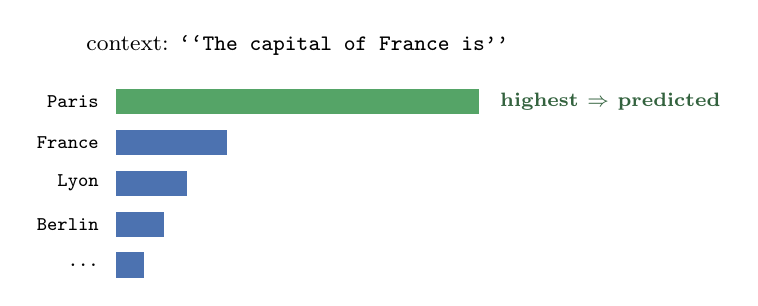
\begin{tikzpicture}
    \node[font=\footnotesize] at (2.4,0.7) {context: \texttt{``The capital of France is''}};
    \foreach \i/\tok/\p in {0/Paris/4.6, 1/France/1.4, 2/Lyon/0.9, 3/Berlin/0.6, 4/\ldots/0.35}{
      \node[left,font=\scriptsize\ttfamily] at (0,-\i*0.52) {\tok};
      \fill[hsbimid] (0.1,-\i*0.52-0.16) rectangle (0.1+\p,-\i*0.52+0.16);
    }
    \fill[cgreen] (0.1,0.16) rectangle (4.7,-0.16);  % highlight Paris (i=0)
    \node[right,font=\scriptsize\bfseries, cgreen!60!black] at (4.85,0) {highest $\Rightarrow$ predicted};
  \end{tikzpicture}
  \end{center}
  {\footnotesize The model never returns ``the answer'' --- it returns a \emph{distribution}. \texttt{temperature} controls how often it picks something other than the top token.}
  \note{%
    \textbf{$\sim$8 min.} Point: the output is a \emph{distribution}, not an answer. This is the slide that explains non-determinism.\\[2pt]
    \textbf{Ask the room:} ``You send the same prompt twice and get different answers. Bug or expected?'' Expected --- and controllable. temperature 0 takes the top token every time; higher temperature samples further down this bar chart.\\[2pt]
    Tie it to practice: \textbf{temperature 0 for extraction and classification} (you want the same answer twice), higher only when you want variety. They will set this parameter constantly from NB 28 onward.\\[2pt]
    Note that even at temperature 0 providers aren't perfectly reproducible --- batching and hardware introduce jitter. Mention only if asked; it's a rabbit hole.
  }
\end{frame}

% ============================================================
\section{Transformer}
% ============================================================
\begin{frame}{The architecture: the Transformer}
  \begin{block}{A stack of attention $+$ feed-forward layers}
    Each token becomes a vector; each layer lets tokens \emph{exchange information} (attention), then transforms each vector (feed-forward). Stack many layers $\to$ rich, context-aware representations.
  \end{block}
  \begin{itemize}
    \item All tokens are processed \emph{in parallel} during training --- a huge speed-up over older recurrent models.
    \item Depth (layers) $+$ width (vector size) $+$ data $=$ the ``large'' in LLM.
  \end{itemize}
  \note{%
    \textbf{$\sim$7 min.} Point: a stack of layers where tokens repeatedly \emph{look at each other} and then get transformed.\\[2pt]
    Pitch this at intuition level --- the next slide has the mechanics. The one structural fact worth stressing is \textbf{parallelism}: unlike the recurrent models it replaced, all tokens are processed at once, which is precisely what made training at this scale affordable.\\[2pt]
    \textbf{If the room is non-technical}, stop here and skip the Q/K/V slide entirely --- it is safely optional, and nothing later in the course depends on it.
  }
\end{frame}

\begin{frame}{The Attention mechanism (Q / K / V)}
  \small
  \begin{center}
  \begin{tabular}{ll}
    \toprule
    \textbf{Step} & \textbf{What happens} \\
    \midrule
    1. Project   & compute Query, Key, Value for every token via learned matrices \\
    2. Score     & $\mathrm{score}_{ij} = Q_i \cdot K_j / \sqrt{d_k}$ \\
    3. Normalise & softmax over $j$ $\to$ weights summing to 1 \\
    4. Mix       & new vector $= \sum_j \mathrm{weight}_{ij}\, V_j$ \\
    \bottomrule
  \end{tabular}
  \end{center}
  \vspace{2pt}
  {\footnotesize $d_k$ is the length of each Key/Query vector; dividing by $\sqrt{d_k}$ keeps scores from blowing up. \textbf{Intuition:} for each word, look at every other word and decide how much to listen to it.}
  \note{%
    \textbf{$\sim$12 min --- the most technical slide in the deck. Optional; cut it first if you are short on time.}\\[2pt]
    Lead with the intuition line at the bottom, \emph{then} the table --- not the other way round.\\[2pt]
    The analogy that works: Query = ``what am I looking for?'', Key = ``what do I offer?'', Value = ``what I actually contribute.'' Scoring Q against K is a relevance match; the softmax turns relevance into a weighting; the mix is a weighted average.\\[2pt]
    \textbf{Worked example on the board:} in ``The animal didn't cross the street because \emph{it} was too tired'', ask what ``it'' should attend to. Attention is what resolves that --- and the answer flips to ``street'' if you change ``tired'' to ``wide''.\\[2pt]
    Don't defend the $\sqrt{d_k}$; it's numerical hygiene, not insight.
  }
\end{frame}

% ============================================================
\section{Using LLMs}
% ============================================================
\begin{frame}{Three levels of using an LLM}
  \begin{center}
  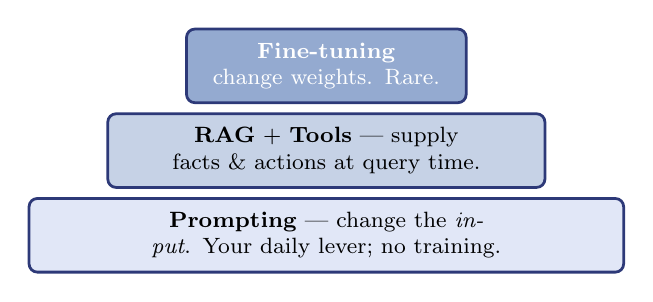
\begin{tikzpicture}
    \node[box, text width=7.2cm, fill=hsbilight]                         (b) {\textbf{Prompting} --- change the \emph{input}. Your daily lever; no training.};
    \node[box, text width=5.2cm, fill=hsbimid!32, above=3pt of b]        (m) {\textbf{RAG $+$ Tools} --- supply facts \& actions at query time.};
    \node[box, text width=3.2cm, fill=hsbimid!60, above=3pt of m, text=white] (t) {\textbf{Fine-tuning}\\ change weights. Rare.};
  \end{tikzpicture}
  \end{center}
  \begin{exampleblock}{Fine-tuning vs RAG}
    Fine-tuning changes \emph{behaviour / style}. \textbf{RAG} (NB 29) keeps the weights frozen and supplies \emph{fresh facts} --- don't fine-tune to add knowledge.
  \end{exampleblock}
  \note{%
    \textbf{$\sim$8 min.} Point: the pyramid is deliberately upside-down in effort --- the widest, cheapest lever (prompting) is the one you'll use 95\,\% of the time.\\[2pt]
    \textbf{The single most valuable correction in this lecture:} ``we'll fine-tune it on our documents'' is almost always wrong. Fine-tuning teaches \emph{behaviour and format}; it is a poor and expensive way to install \emph{facts}, which go stale the day after you train. Facts belong in retrieval.\\[2pt]
    \textbf{Ask the room:} ``You want the bot to answer from your 400-page handbook. Which level?'' RAG --- and if anyone says fine-tune, this is the moment to unpick it.\\[2pt]
    Forward-reference NB 29 (RAG) and NB 30 (tools) so it lands as a roadmap, not a taxonomy.
  }
\end{frame}

\begin{frame}{Five prompting techniques}
  \small
  \begin{center}
  \begin{tabular}{lp{7.0cm}}
    \toprule
    \textbf{Technique} & \textbf{When to reach for it} \\
    \midrule
    Zero-shot          & a general question; you trust the defaults \\
    Few-shot           & you want a \emph{consistent} format --- show 2--3 examples \\
    Chain-of-Thought   & multi-step reasoning --- ask it to work step by step \\
    Role assignment    & set tone / depth --- ``you are a senior analyst\ldots'' \\
    Format constraint  & machine-parseable output --- ``return JSON with keys\ldots'' \\
    \bottomrule
  \end{tabular}
  \end{center}
  {\footnotesize A production prompt stacks several: \emph{role} $+$ \emph{context} $+$ \emph{task} $+$ \emph{format} $+$ \emph{constraints}.}
  \note{%
    \textbf{$\sim$10 min --- make this the interactive one.}\\[2pt]
    Don't lecture the table. Take a deliberately bad prompt (``summarise this'') and improve it live with the room, adding one technique at a time until it's role $+$ context $+$ task $+$ format $+$ constraints. They should watch the output get sharper at each step.\\[2pt]
    \textbf{Format constraint is the one with engineering consequences:} ``return JSON with keys x, y'' is what makes an LLM callable as a \emph{function} rather than a chat toy --- that's the whole premise of NB 28.\\[2pt]
    Honest caveat on chain-of-thought: on newer reasoning models, explicitly asking for step-by-step adds less than it used to --- they already do it internally.
  }
\end{frame}

% ============================================================
\section{Limits}
% ============================================================
\begin{frame}{Two structural limitations}
  \begin{alertblock}{1. Hallucinations}
    The model predicts \emph{plausible} continuations, not \emph{true} ones --- so it can invent clauses, statistics, or APIs with full confidence.
  \end{alertblock}
  \begin{alertblock}{2. Knowledge cutoff}
    It knows nothing after its training date, and nothing about your \emph{private} data --- no current prices, no internal reports.
  \end{alertblock}
  \begin{exampleblock}{Mitigations (built later in the course)}
    \textbf{RAG} (NB 29) grounds answers in evidence $\cdot$ \textbf{Tools} (NB 30) let it look things up $\cdot$ \textbf{Evaluation} (NB 32) measures how often it's wrong.
  \end{exampleblock}
  \note{%
    \textbf{$\sim$10 min + close.} Point: both limitations are \emph{structural}, not bugs awaiting a patch --- they fall straight out of ``predicts plausible continuations.'' Close the loop with slide 1 explicitly.\\[2pt]
    Frame hallucination precisely: the model is not lying and does not know it is wrong. Nothing in the objective ever rewarded truth --- only plausibility.\\[2pt]
    \textbf{The professional habit to leave them with:} never ask ``is it accurate?'' --- ask ``\emph{how would I measure} how often it's wrong, and what happens when it is?'' That reframing is the bridge to NB 32 and to Module 18.\\[2pt]
    \textbf{Send them to Notebook 27} --- it runs entirely offline against the MockLLM, so nobody needs an API key to start.
  }
\end{frame}

\end{document}
"
\ifdefined\notesmode
  \usepackage{pgfpages}
  \setbeameroption{show notes on second screen=right}
\fi

\usetheme{Madrid}
\usecolortheme{default}
\setbeamertemplate{navigation symbols}{}
\setbeamertemplate{footline}[frame number]
\setbeamertemplate{blocks}[rounded][shadow=false]
\setbeamertemplate{headline}{%
  \leavevmode%
  \hbox{%
    \begin{beamercolorbox}[wd=\paperwidth,ht=2.5ex,dp=1.125ex]{section in head/foot}%
      \insertsectionnavigationhorizontal{\paperwidth}{}{\hskip0pt plus1filll}%
    \end{beamercolorbox}%
  }%
}
\AtBeginSection[]{%
  \begin{frame}{Outline}
    \tableofcontents[currentsection,sectionstyle=show/shaded,subsectionstyle=show/show/hide]
  \end{frame}
}

\definecolor{hsbiblue}{RGB}{45,57,120}
\definecolor{hsbimid}{RGB}{76,114,176}
\definecolor{hsbilight}{RGB}{225,231,247}
\definecolor{cgreen}{RGB}{85,164,103}
\definecolor{corange}{RGB}{221,132,82}
\definecolor{cred}{RGB}{196,78,82}
\definecolor{cpurple}{RGB}{129,114,178}
\tikzset{
  box/.style={rounded corners=3pt, draw=hsbiblue, line width=1pt, fill=hsbilight, align=center, inner sep=5pt, font=\footnotesize},
  tok/.style={rounded corners=2pt, draw=hsbiblue, line width=1pt, fill=hsbimid!22, align=center, minimum height=0.7cm, inner xsep=4pt, font=\footnotesize\ttfamily},
  arr/.style={-{Stealth[length=2.6mm]}, line width=1pt, draw=hsbiblue},
}

\title{LLM Fundamentals}
\subtitle{Module 8 --- AI Engineering $\cdot$ Notebook 27}
\author{Prof.\ Dr.\ Christoph Weisser}
\institute{HSBI}
\date{Summer Semester 2026}

\begin{document}

\begin{frame}\titlepage\end{frame}

\begin{frame}{Contents}
  \tableofcontents[hideallsubsections]
\end{frame}

% ============================================================
\section{Tokens}
% ============================================================
\begin{frame}{What is a Large Language Model?}
  \begin{block}{A next-token predictor}
    An LLM learns statistical relationships between words from massive corpora. Given some text, it computes the \emph{most probable continuation}, one token at a time.
  \end{block}
  \begin{exampleblock}{Analogy}
    Someone who has read every book ever written: they can continue any topic plausibly --- but have \emph{no built-in sense} of what is true, current, or private to your company.
  \end{exampleblock}
  \note{%
    \textbf{$\sim$6 min --- the framing for the whole lecture.}\\[2pt]
    Point: everything surprising about LLMs (hallucination, cutoff, prompt sensitivity) follows from \emph{one} fact --- it predicts the next token. Say that now; you will call back to it on every remaining slide.\\[2pt]
    \textbf{Ask the room:} ``If it only predicts likely text, why does it ever get facts right?'' Answer: true statements are common in the training data, so plausibility and truth correlate --- but only correlate. That gap is the entire second half of this lecture.\\[2pt]
    \textbf{Resist} defining tokens, attention or temperature here --- they each get their own slide.
  }
\end{frame}

\begin{frame}{How LLMs see text: tokens}
  \begin{center}
  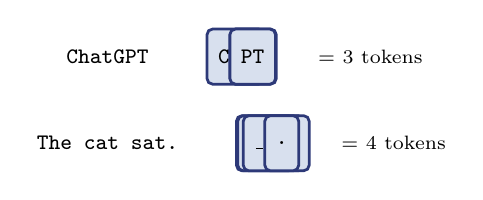
\begin{tikzpicture}[node distance=2pt]
    \node[font=\footnotesize] (l1) at (-3.0,0.55) {\texttt{ChatGPT}};
    \node[tok, right=0.6cm of l1] (t1) {Chat};
    \node[tok, right of=t1] (t2) {G};
    \node[tok, right of=t2] (t3) {PT};
    \node[font=\scriptsize, right=0.4cm of t3] {= 3 tokens};
    \node[font=\footnotesize] (l2) at (-3.0,-0.55) {\texttt{The cat sat.}};
    \node[tok, right=0.6cm of l2] (u1) {The};
    \node[tok, right of=u1] (u2) {\_cat};
    \node[tok, right of=u2] (u3) {\_sat};
    \node[tok, right of=u3] (u4) {.};
    \node[font=\scriptsize, right=0.4cm of u4] {= 4 tokens};
  \end{tikzpicture}
  \end{center}
  \begin{itemize}
    \item Cost and the \textbf{context window} are measured in tokens --- not characters, not words.
    \item Rule of thumb: 1 English token $\approx$ 4 characters $\approx$ 0.75 words ($1{,}000$ tokens $\approx$ 750 words).
    \item Code and non-English text tokenize \emph{less} efficiently; the model is blind to characters \emph{within} a token (``how many r's in strawberry?'').
  \end{itemize}
  \note{%
    \textbf{$\sim$10 min.} Point: tokens are the unit of \emph{cost}, \emph{context} and \emph{blindness}.\\[2pt]
    The strawberry example is the one they'll remember --- the model can't count letters it never sees separately. Ask it live if you have a provider configured; it fails convincingly.\\[2pt]
    \textbf{Ask the room:} ``Your prompt is 2{,}000 words. Roughly how many tokens, and does it fit?'' ($\approx$2{,}700 --- fits anywhere today.) The arithmetic matters because they'll be paying per token in Module 8.\\[2pt]
    \textbf{Non-English matters here:} German compounds tokenize badly, so the same text costs noticeably more than in English. Worth naming for a German-speaking cohort.
  }
\end{frame}

\begin{frame}{What are parameters? Why ``large''?}
  \small
  \begin{center}
  \begin{tabular}{llr}
    \toprule
    \textbf{Model} & \textbf{Parameters} & \textbf{Year} \\
    \midrule
    GPT-2                              & 1.5 billion                  & 2019 \\
    Llama-3 (open-weights)             & 8B / 70B / 405B              & 2024 \\
    Frontier (GPT-5.x, Claude, Gemini) & hundreds of billions (est.)  & 2023+ \\
    \bottomrule
  \end{tabular}
  \end{center}
  \begin{alertblock}{Key insight}
    There is \emph{no} manual list of facts inside the model. Knowledge is \emph{implicitly distributed} across all the weights --- which is exactly why it can be confidently wrong.
  \end{alertblock}
  \note{%
    \textbf{$\sim$7 min.} Point: parameters are learned weights, not stored facts. There is no row in a table saying ``Paris is the capital of France.''\\[2pt]
    That is \emph{why} you cannot patch a wrong fact by editing something, and why the fix is RAG (retrieval), not surgery on the model.\\[2pt]
    \textbf{Keep the numbers loose} --- frontier parameter counts are estimates and they date fast. The trend is the teaching point, not the figures.\\[2pt]
    \textbf{Ask the room:} ``Where inside the model is the fact stored?'' The honest answer --- smeared across billions of weights, nowhere in particular --- is genuinely unsettling and should be.
  }
\end{frame}

% ============================================================
\section{Training}
% ============================================================
\begin{frame}{The training objective: next-token prediction}
  \begin{block}{Hide $\to$ predict $\to$ measure $\to$ nudge, trillions of times}
    Hide the next token, ask the model to predict it, measure the error, nudge every parameter slightly toward a better prediction.
  \end{block}
  \[
    \mathcal{L} \;=\; -\sum_i y_i \log \hat{p}_i
  \]
  where $y_i = 1$ for the one true next token and $0$ otherwise (a \emph{one-hot} target), and $\hat{p}_i$ is the model's predicted probability for token $i$. Grammar, facts, and reasoning emerge as \emph{side-effects}.

  \vspace{2pt}
  {\footnotesize You write this exact loop --- loss $\to$ backward $\to$ step --- yourself in \textbf{Module 6 (PyTorch)}; an LLM trains with the same five moves, just with more parameters and more data.}
  \note{%
    \textbf{$\sim$10 min.} Point: the objective is embarrassingly simple, and everything impressive is a \emph{side-effect} of doing it at scale.\\[2pt]
    Don't derive the cross-entropy. Read it in words: ``the loss is small when the probability assigned to the token that actually came next is large.'' That sentence is the whole equation.\\[2pt]
    \textbf{The call-forward matters:} if your cohort is doing Module 6, promise them they will write this exact loop in PyTorch. It demystifies the whole thing --- same five moves, more data.\\[2pt]
    \textbf{Misconception to kill:} that the model was ``taught'' grammar or facts. Nobody labelled anything --- the text was its own label.
  }
\end{frame}

\begin{frame}{The output is a probability over \emph{every} token}
  \begin{center}
  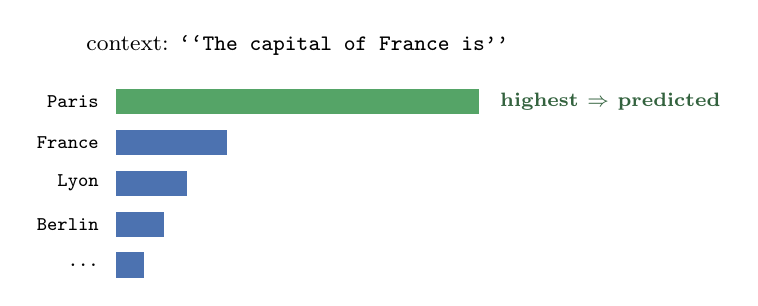
\begin{tikzpicture}
    \node[font=\footnotesize] at (2.4,0.7) {context: \texttt{``The capital of France is''}};
    \foreach \i/\tok/\p in {0/Paris/4.6, 1/France/1.4, 2/Lyon/0.9, 3/Berlin/0.6, 4/\ldots/0.35}{
      \node[left,font=\scriptsize\ttfamily] at (0,-\i*0.52) {\tok};
      \fill[hsbimid] (0.1,-\i*0.52-0.16) rectangle (0.1+\p,-\i*0.52+0.16);
    }
    \fill[cgreen] (0.1,0.16) rectangle (4.7,-0.16);  % highlight Paris (i=0)
    \node[right,font=\scriptsize\bfseries, cgreen!60!black] at (4.85,0) {highest $\Rightarrow$ predicted};
  \end{tikzpicture}
  \end{center}
  {\footnotesize The model never returns ``the answer'' --- it returns a \emph{distribution}. \texttt{temperature} controls how often it picks something other than the top token.}
  \note{%
    \textbf{$\sim$8 min.} Point: the output is a \emph{distribution}, not an answer. This is the slide that explains non-determinism.\\[2pt]
    \textbf{Ask the room:} ``You send the same prompt twice and get different answers. Bug or expected?'' Expected --- and controllable. temperature 0 takes the top token every time; higher temperature samples further down this bar chart.\\[2pt]
    Tie it to practice: \textbf{temperature 0 for extraction and classification} (you want the same answer twice), higher only when you want variety. They will set this parameter constantly from NB 28 onward.\\[2pt]
    Note that even at temperature 0 providers aren't perfectly reproducible --- batching and hardware introduce jitter. Mention only if asked; it's a rabbit hole.
  }
\end{frame}

% ============================================================
\section{Transformer}
% ============================================================
\begin{frame}{The architecture: the Transformer}
  \begin{block}{A stack of attention $+$ feed-forward layers}
    Each token becomes a vector; each layer lets tokens \emph{exchange information} (attention), then transforms each vector (feed-forward). Stack many layers $\to$ rich, context-aware representations.
  \end{block}
  \begin{itemize}
    \item All tokens are processed \emph{in parallel} during training --- a huge speed-up over older recurrent models.
    \item Depth (layers) $+$ width (vector size) $+$ data $=$ the ``large'' in LLM.
  \end{itemize}
  \note{%
    \textbf{$\sim$7 min.} Point: a stack of layers where tokens repeatedly \emph{look at each other} and then get transformed.\\[2pt]
    Pitch this at intuition level --- the next slide has the mechanics. The one structural fact worth stressing is \textbf{parallelism}: unlike the recurrent models it replaced, all tokens are processed at once, which is precisely what made training at this scale affordable.\\[2pt]
    \textbf{If the room is non-technical}, stop here and skip the Q/K/V slide entirely --- it is safely optional, and nothing later in the course depends on it.
  }
\end{frame}

\begin{frame}{The Attention mechanism (Q / K / V)}
  \small
  \begin{center}
  \begin{tabular}{ll}
    \toprule
    \textbf{Step} & \textbf{What happens} \\
    \midrule
    1. Project   & compute Query, Key, Value for every token via learned matrices \\
    2. Score     & $\mathrm{score}_{ij} = Q_i \cdot K_j / \sqrt{d_k}$ \\
    3. Normalise & softmax over $j$ $\to$ weights summing to 1 \\
    4. Mix       & new vector $= \sum_j \mathrm{weight}_{ij}\, V_j$ \\
    \bottomrule
  \end{tabular}
  \end{center}
  \vspace{2pt}
  {\footnotesize $d_k$ is the length of each Key/Query vector; dividing by $\sqrt{d_k}$ keeps scores from blowing up. \textbf{Intuition:} for each word, look at every other word and decide how much to listen to it.}
  \note{%
    \textbf{$\sim$12 min --- the most technical slide in the deck. Optional; cut it first if you are short on time.}\\[2pt]
    Lead with the intuition line at the bottom, \emph{then} the table --- not the other way round.\\[2pt]
    The analogy that works: Query = ``what am I looking for?'', Key = ``what do I offer?'', Value = ``what I actually contribute.'' Scoring Q against K is a relevance match; the softmax turns relevance into a weighting; the mix is a weighted average.\\[2pt]
    \textbf{Worked example on the board:} in ``The animal didn't cross the street because \emph{it} was too tired'', ask what ``it'' should attend to. Attention is what resolves that --- and the answer flips to ``street'' if you change ``tired'' to ``wide''.\\[2pt]
    Don't defend the $\sqrt{d_k}$; it's numerical hygiene, not insight.
  }
\end{frame}

% ============================================================
\section{Using LLMs}
% ============================================================
\begin{frame}{Three levels of using an LLM}
  \begin{center}
  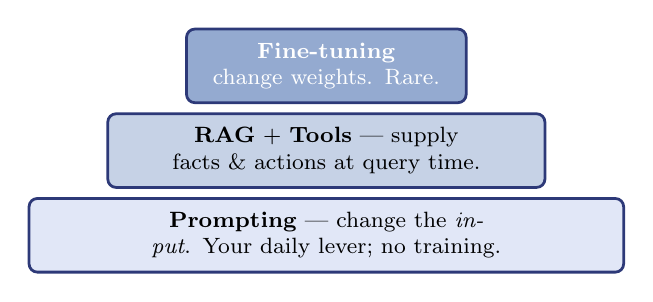
\begin{tikzpicture}
    \node[box, text width=7.2cm, fill=hsbilight]                         (b) {\textbf{Prompting} --- change the \emph{input}. Your daily lever; no training.};
    \node[box, text width=5.2cm, fill=hsbimid!32, above=3pt of b]        (m) {\textbf{RAG $+$ Tools} --- supply facts \& actions at query time.};
    \node[box, text width=3.2cm, fill=hsbimid!60, above=3pt of m, text=white] (t) {\textbf{Fine-tuning}\\ change weights. Rare.};
  \end{tikzpicture}
  \end{center}
  \begin{exampleblock}{Fine-tuning vs RAG}
    Fine-tuning changes \emph{behaviour / style}. \textbf{RAG} (NB 29) keeps the weights frozen and supplies \emph{fresh facts} --- don't fine-tune to add knowledge.
  \end{exampleblock}
  \note{%
    \textbf{$\sim$8 min.} Point: the pyramid is deliberately upside-down in effort --- the widest, cheapest lever (prompting) is the one you'll use 95\,\% of the time.\\[2pt]
    \textbf{The single most valuable correction in this lecture:} ``we'll fine-tune it on our documents'' is almost always wrong. Fine-tuning teaches \emph{behaviour and format}; it is a poor and expensive way to install \emph{facts}, which go stale the day after you train. Facts belong in retrieval.\\[2pt]
    \textbf{Ask the room:} ``You want the bot to answer from your 400-page handbook. Which level?'' RAG --- and if anyone says fine-tune, this is the moment to unpick it.\\[2pt]
    Forward-reference NB 29 (RAG) and NB 30 (tools) so it lands as a roadmap, not a taxonomy.
  }
\end{frame}

\begin{frame}{Five prompting techniques}
  \small
  \begin{center}
  \begin{tabular}{lp{7.0cm}}
    \toprule
    \textbf{Technique} & \textbf{When to reach for it} \\
    \midrule
    Zero-shot          & a general question; you trust the defaults \\
    Few-shot           & you want a \emph{consistent} format --- show 2--3 examples \\
    Chain-of-Thought   & multi-step reasoning --- ask it to work step by step \\
    Role assignment    & set tone / depth --- ``you are a senior analyst\ldots'' \\
    Format constraint  & machine-parseable output --- ``return JSON with keys\ldots'' \\
    \bottomrule
  \end{tabular}
  \end{center}
  {\footnotesize A production prompt stacks several: \emph{role} $+$ \emph{context} $+$ \emph{task} $+$ \emph{format} $+$ \emph{constraints}.}
  \note{%
    \textbf{$\sim$10 min --- make this the interactive one.}\\[2pt]
    Don't lecture the table. Take a deliberately bad prompt (``summarise this'') and improve it live with the room, adding one technique at a time until it's role $+$ context $+$ task $+$ format $+$ constraints. They should watch the output get sharper at each step.\\[2pt]
    \textbf{Format constraint is the one with engineering consequences:} ``return JSON with keys x, y'' is what makes an LLM callable as a \emph{function} rather than a chat toy --- that's the whole premise of NB 28.\\[2pt]
    Honest caveat on chain-of-thought: on newer reasoning models, explicitly asking for step-by-step adds less than it used to --- they already do it internally.
  }
\end{frame}

% ============================================================
\section{Limits}
% ============================================================
\begin{frame}{Two structural limitations}
  \begin{alertblock}{1. Hallucinations}
    The model predicts \emph{plausible} continuations, not \emph{true} ones --- so it can invent clauses, statistics, or APIs with full confidence.
  \end{alertblock}
  \begin{alertblock}{2. Knowledge cutoff}
    It knows nothing after its training date, and nothing about your \emph{private} data --- no current prices, no internal reports.
  \end{alertblock}
  \begin{exampleblock}{Mitigations (built later in the course)}
    \textbf{RAG} (NB 29) grounds answers in evidence $\cdot$ \textbf{Tools} (NB 30) let it look things up $\cdot$ \textbf{Evaluation} (NB 32) measures how often it's wrong.
  \end{exampleblock}
  \note{%
    \textbf{$\sim$10 min + close.} Point: both limitations are \emph{structural}, not bugs awaiting a patch --- they fall straight out of ``predicts plausible continuations.'' Close the loop with slide 1 explicitly.\\[2pt]
    Frame hallucination precisely: the model is not lying and does not know it is wrong. Nothing in the objective ever rewarded truth --- only plausibility.\\[2pt]
    \textbf{The professional habit to leave them with:} never ask ``is it accurate?'' --- ask ``\emph{how would I measure} how often it's wrong, and what happens when it is?'' That reframing is the bridge to NB 32 and to Module 18.\\[2pt]
    \textbf{Send them to Notebook 27} --- it runs entirely offline against the MockLLM, so nobody needs an API key to start.
  }
\end{frame}

\end{document}
